\documentclass{homework}
\usepackage{homework}
\usepackage{hanhua}
\title{Week 4}
\date{}
\begin{document}
\maketitle
\section{用Taylor级数法(q=2,3)计算$\frac{\mathrm{d}u}{\mathrm{d}t}=u-u^2$,并与Euler显格式比较(P74/1)}
代码如下:
\lstinputlisting[language=Matlab]{Taylor.m}
Euler显式格式即当q=1时的Taylor级数法。
得到的误差比较如下:
\begin{figure}[H]
\hspace{-5em}
\begin{subfigure}[t]{0.6\textwidth}
\centering
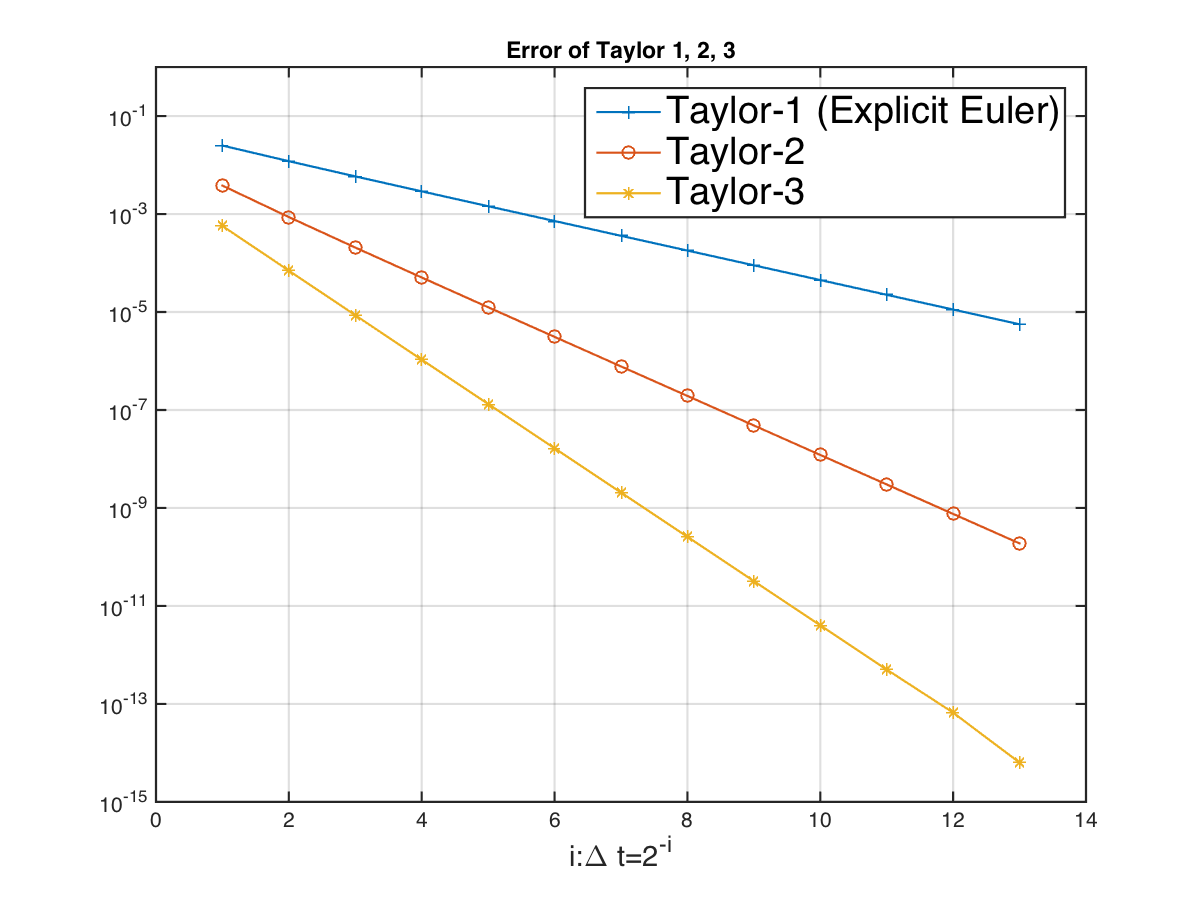
\includegraphics[width=\textwidth]{Taylor.png}
\end{subfigure}
\begin{subfigure}[t]{0.6\textwidth}
\centering
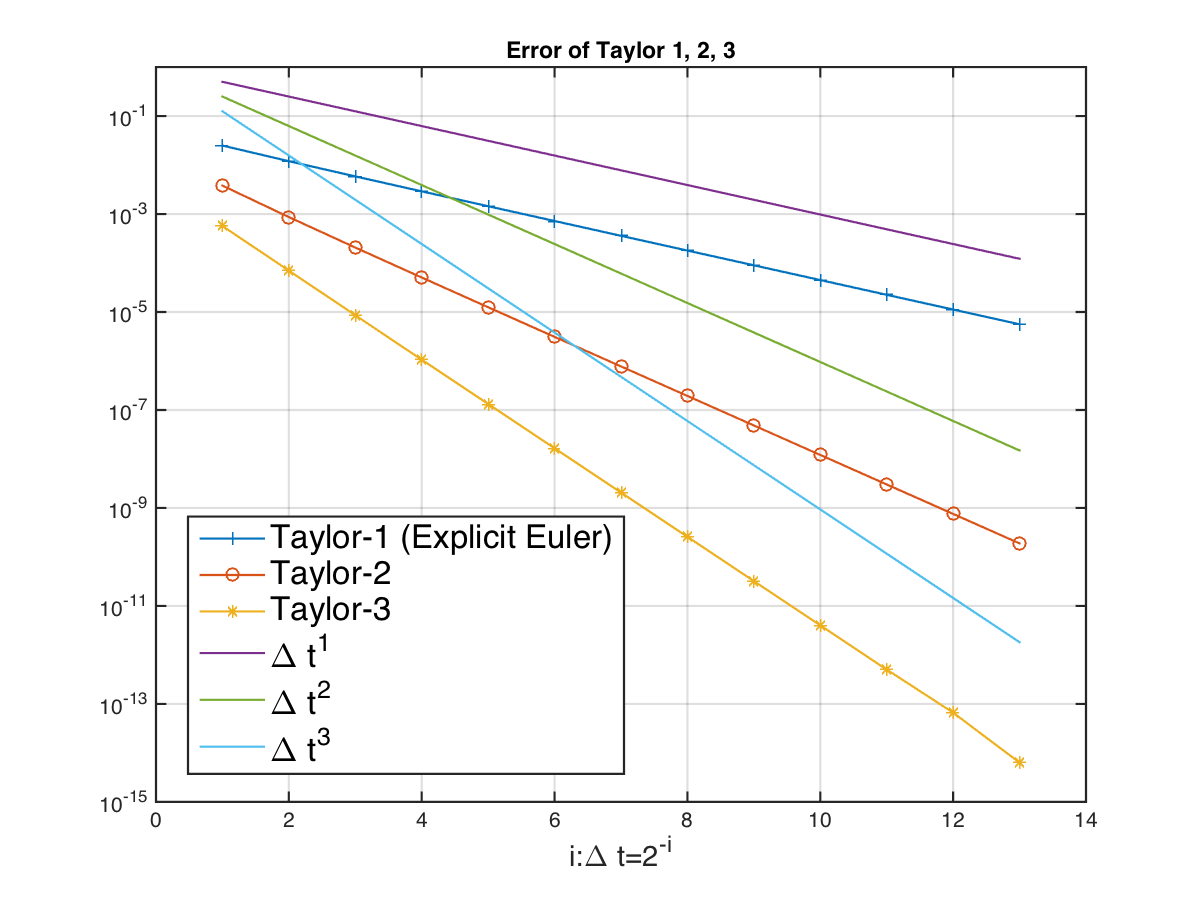
\includegraphics[width=\textwidth]{TwithD.png}
\end{subfigure}
\end{figure}
将$\Delta t^1,\Delta t^2,\Delta t^3$画出可以由平行关系看出各方法的收敛阶数。或者通过分别枚举p=1,2,3,4,并将每种方法得到的结果代入$$\frac{\bigabs{u(t)-u_n}}{\Delta t^p},$$可以得到最高的具有常数上界结果的p即其收敛阶数:
\begin{figure}[H]
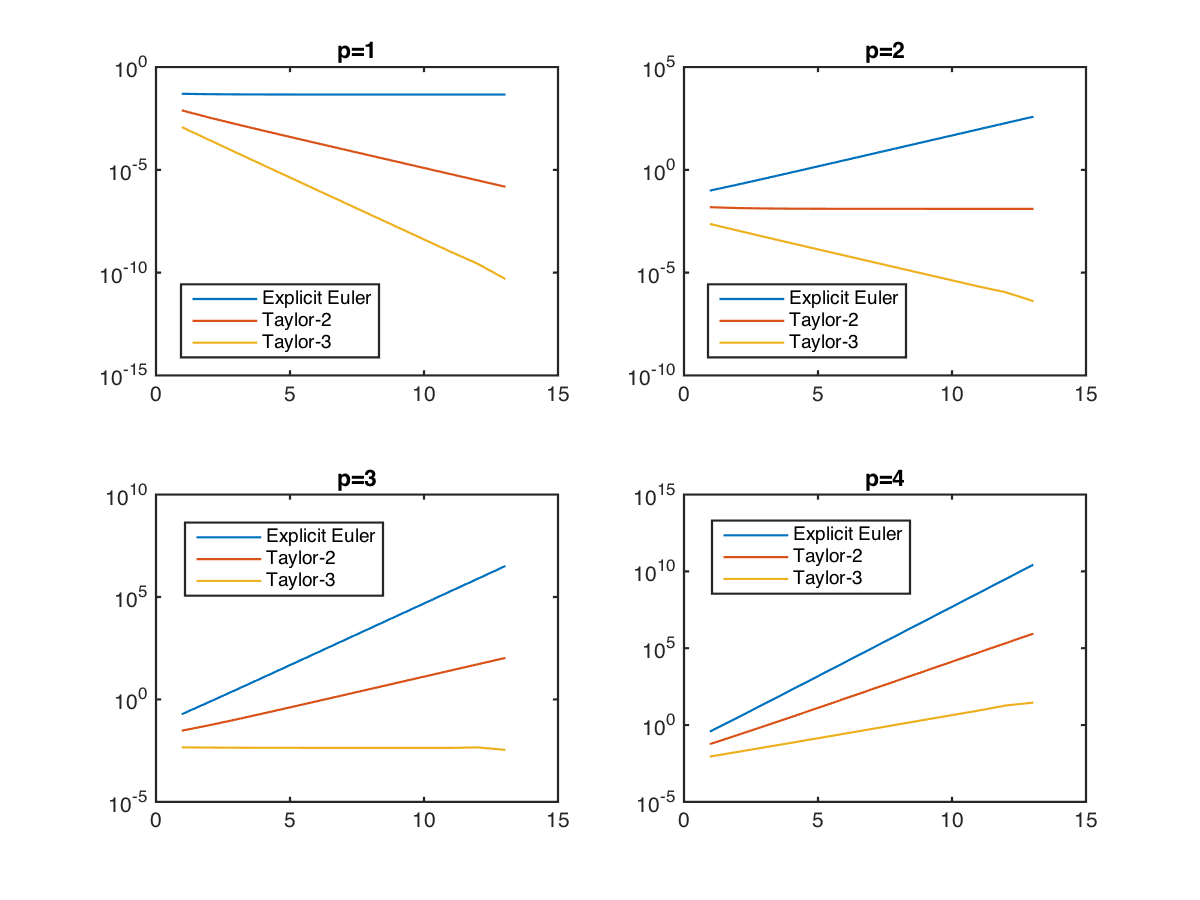
\includegraphics[width=0.9\linewidth]{TsepP.png}
\centering
\end{figure}
可以看出,显式欧拉格式、2阶、3阶Taylor级数法的收敛阶数分别为1、2、3。
\section{用一到四阶格式的Runge-Kutta方法计算$\frac{\mathrm{d}u}{\mathrm{d}t}=u-u^2$,观察收敛阶(P79/3)}
代码如下:
\lstinputlisting[language=Matlab]{RungeKutta.m}
Euler显式格式即当q=1时的Runge-Kutta方法。4阶采用的是3/8的Kutta方法。

得到的误差比较如下图,可以看出4阶Kutta方法在步长为$2^{-10}$时误差就达到了$10^{-15}$的数量级,已经接近机器精度了,再减小步长已经不能提高精度了。
\begin{figure}[H]
\hspace{-5em}
\begin{subfigure}[t]{0.6\textwidth}
\centering
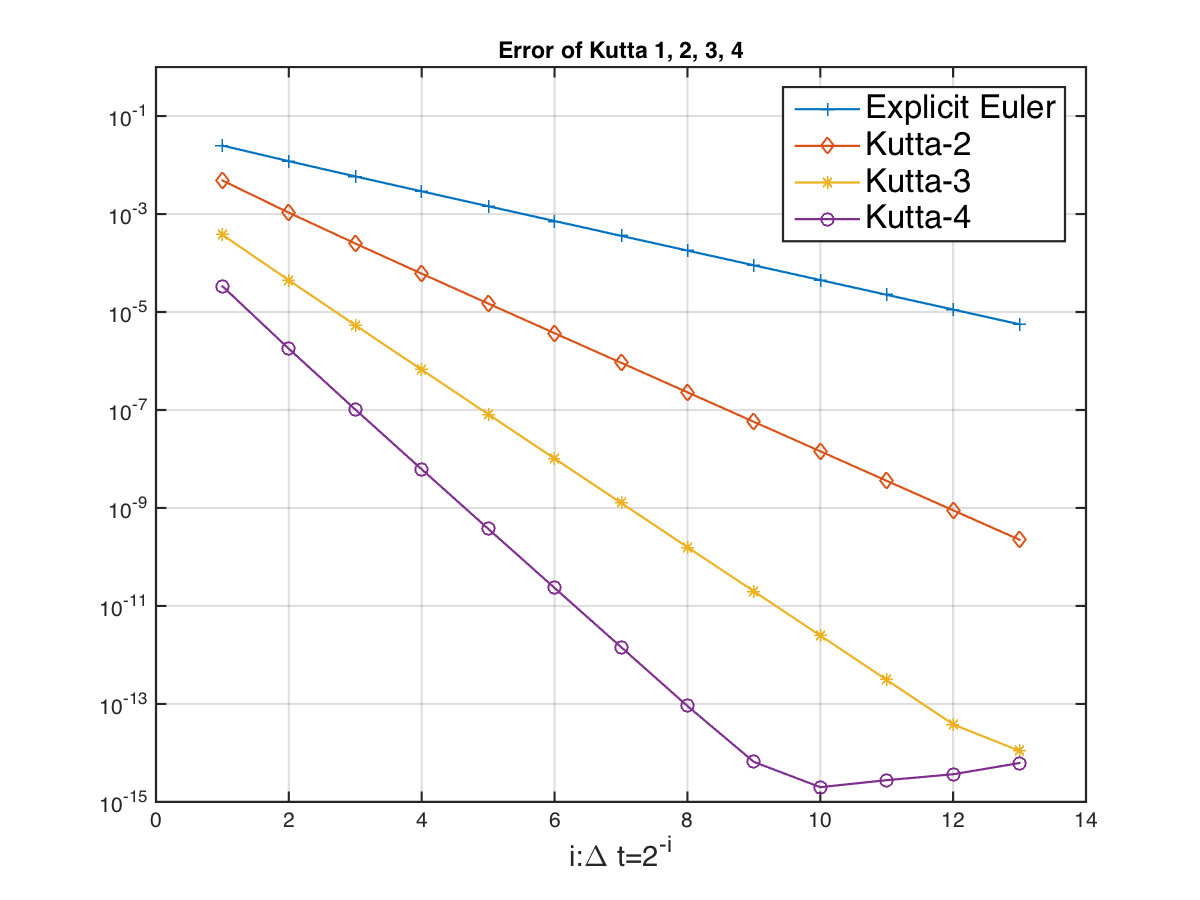
\includegraphics[width=\textwidth]{RungeKutta.png}
\end{subfigure}
\begin{subfigure}[t]{0.6\textwidth}
\centering
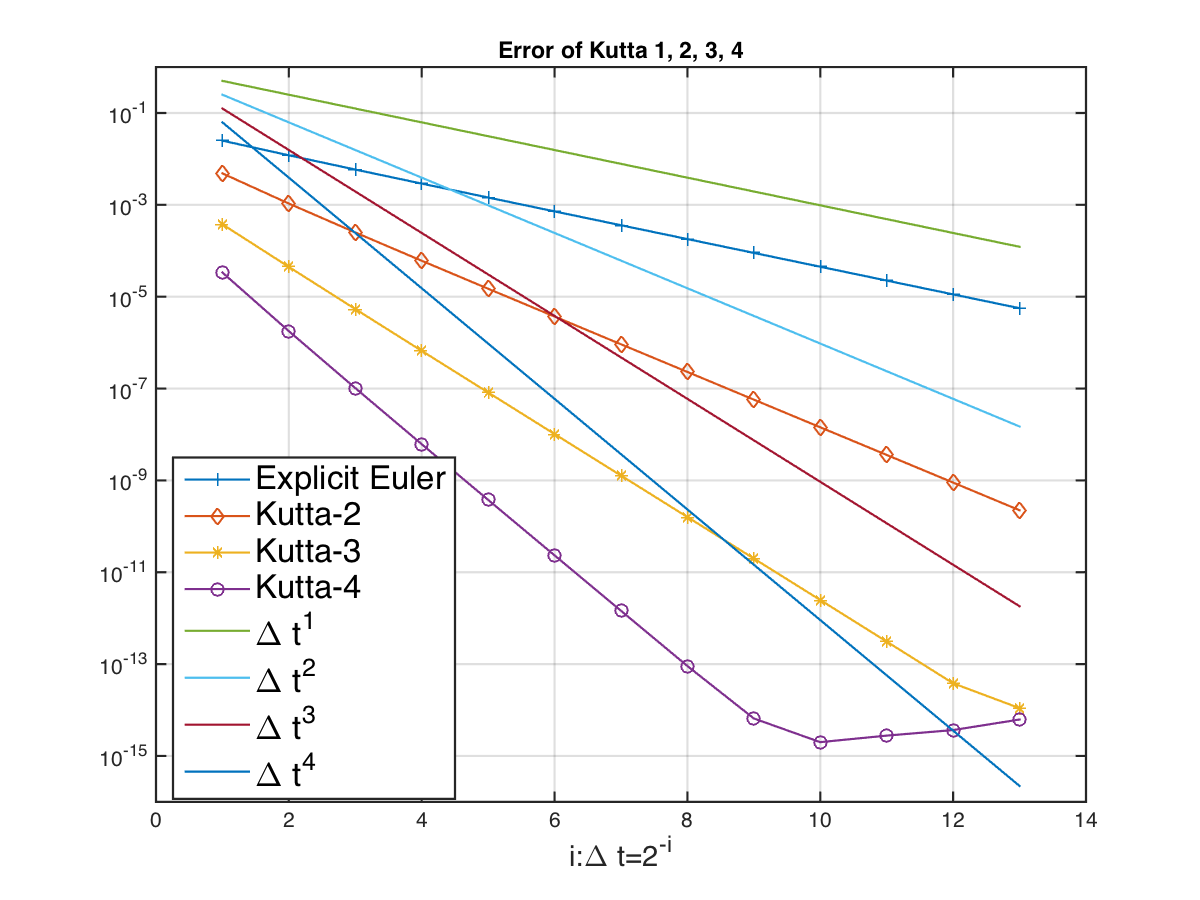
\includegraphics[width=\textwidth]{RKwithD.png}
\end{subfigure}
\end{figure}
同样可通过两种方法考察其收敛阶数各为多少:
\begin{figure}[H]
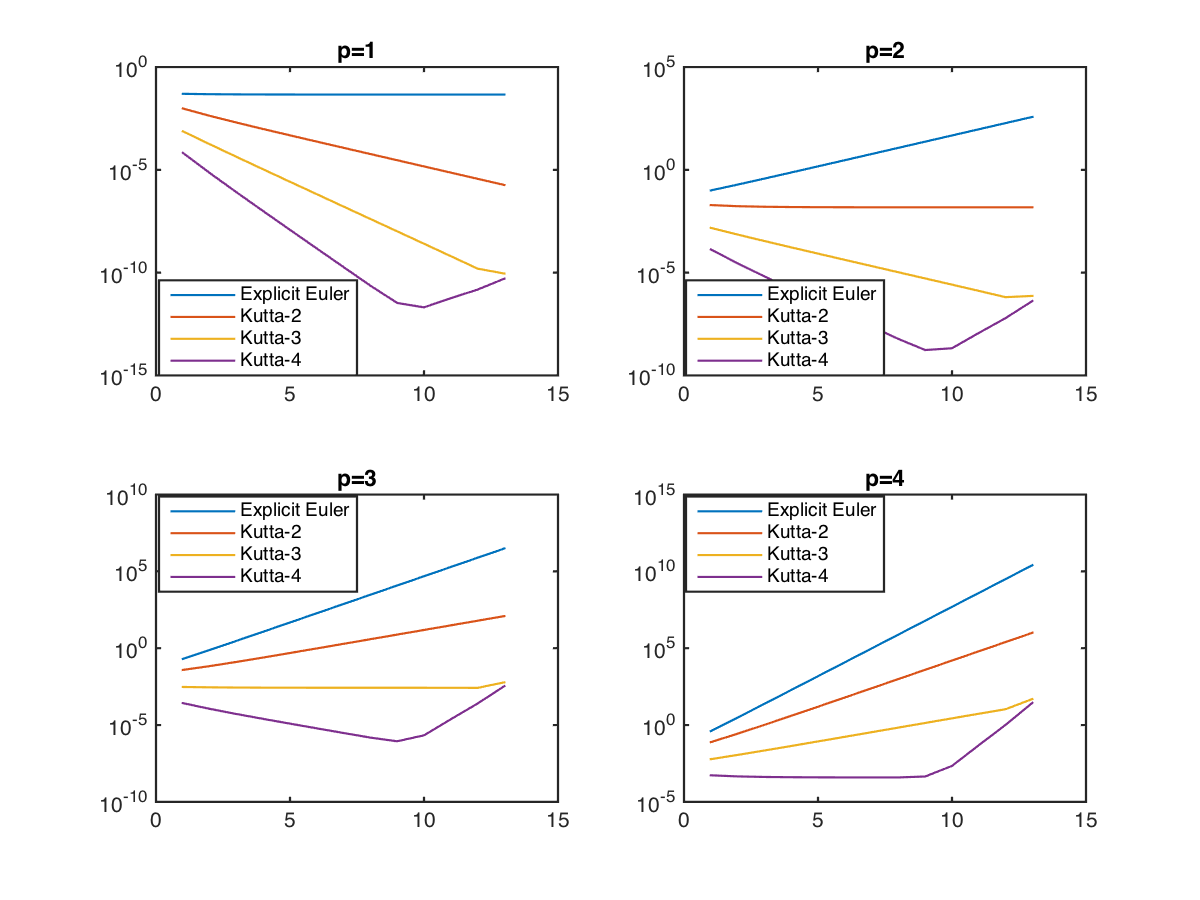
\includegraphics[width=0.9\linewidth]{RKsepP.png}
\centering
\end{figure}
可以看出,显式欧拉格式、2阶、3阶、4阶Kutta方法的收敛阶数分别为1、2、3、4。
\end{document}
